\chapter{Fundamentação e desenvolvimentos teóricos}
\label{chap:fundamentacao}


\section{Campo de indução magnética}
\label{sec:campo}

De acordo com as leis da magnetostática, um conjunto de fontes magnéticas arbitrárias produz, 
na ausência de densidades de corrente, um campo de indução magnética dado por 
\citep[e.g., ][ p. 175, 193]{jackson1975}:
\begin{equation}
\mathbf{B}(x, y, z) = - \boldsymbol{\nabla} \Gamma(x, y, z) \: ,
\label{eq:B-true-generic}
\end{equation}
em que 
\begin{equation}
\Gamma(x, y, z) = - \gamma_{m} \iiint\limits_{\upsilon} \mathbf{m}(x', y', z') \cdot \boldsymbol{\nabla} \frac{1}{r'} 
\; d\upsilon'
\label{eq:Gamma-potential}
\end{equation}
é o potencial magnético escalar, $(x', y', z')$ representa um ponto localizado no interior do 
volume $\upsilon$ das fontes, 
\begin{equation}
\frac{1}{r'} = \frac{1}{\left[ (x - x')^{2} + (y - y')^{2} + (z - z')^{2} \right]^{\frac{1}{2}}}
\label{eq:inv-r'}
\end{equation}
é a função inverso da distância entre um ponto $(x', y', z')$ e um ponto $(x, y, z)$ localizado fora
das fontes e 
\begin{equation}
\mathbf{m}(x', y', z') = \begin{bmatrix}
m_{x}(x', y', z') \\
m_{y}(x', y', z') \\
m_{z}(x', y', z')
\end{bmatrix}
\label{eq:mag-vector-true-generic}
\end{equation}
é o vetor magnetização no interior das fontes.
A partir das equações acima, a componente $\alpha$, $\alpha = x, y, z$ do campo de indução 
magnética produzido pelas fontes é dada por
\begin{equation}
B_{\alpha}(x, y, z) = \gamma_{m} \iiint\limits_{\upsilon} 
\mathbf{m}(x', y', z') \cdot \partial_{\alpha} \boldsymbol{\nabla} \frac{1}{r'} 
\; d\upsilon' \: , \quad \alpha = x, y, z \: ,
\label{eq:B-alpha-true-generic}
\end{equation}
em que $\partial_{\alpha} \equiv \frac{\partial}{\partial \alpha}$ representa 
a derivada parcial em relação a coordenada $\alpha = x, y, z$.
Além disso, nestas condições, o campo de indução magnética $\mathbf{B}(x, y, z)$ (equação \ref{eq:B-true-generic}) 
é governado pela lei de Gauss para campos magnéticos
\begin{equation}
\boldsymbol{\nabla} \cdot \mathbf{B}(x, y, z) = 
\partial_{x} B_{x}(x, y, z) + \partial_{y} B_{y}(x, y, z) + \partial_{z} B_{z}(x, y, z) = 
0
\label{eq:lei-Gauss}
\end{equation}
e a lei de Ampère
\begin{equation}
\boldsymbol{\nabla} \times \mathbf{B}(x, y, z) = \begin{bmatrix}
\partial_{y} B_{z}(x, y, z) - \partial_{z} B_{y}(x, y, z) \\
\partial_{z} B_{x}(x, y, z) - \partial_{x} B_{z}(x, y, z) \\
\partial_{x} B_{y}(x, y, z) - \partial_{y} B_{x}(x, y, z) 
\end{bmatrix} = 
\begin{bmatrix}
0 \\
0 \\
0
\end{bmatrix} \: .
\label{eq:lei-Ampere}
\end{equation}

Usando as equações do campo de indução magnética produzido por um conjunto de fontes 
magnéticas arbitrárias, é possível definir uma importante quantidade utilizada em  
geofísica aplicada denominada a \textit{anomalia de campo total}. Esta quantidade é
comumente definida da seguinte forma \citep[][ p. 179]{blakely1996}:
\begin{equation}
\Delta T(x, y, z) = \hat{\mathbf{u}}(I_{0}, D_{0}) \cdot \mathbf{B}(x, y, z) \: ,
\label{eq:Delta-T-true}
\end{equation}
em que $I_{0}$ e $D_{0}$ são a inclinação e a declinação do campo principal na área de 
estudo, respectivamente, e $\hat{\mathbf{u}}(I_{0}, D_{0})$ é um vetor unitário definido  
pela função vetorial
\begin{equation}
\hat{\mathbf{u}}(I, D) = 
\begin{bmatrix}
\hat{u}_{x}(I, D) \\
\hat{u}_{y}(I, D) \\
\hat{u}_{z}(I, D) 
\end{bmatrix} = 
\begin{bmatrix}
\cos I \, \cos D \\
\cos I \, \sin D \\
\sin I
\end{bmatrix} \: ,
\label{eq:u-hat}
\end{equation}
para o caso particular em que $I = I_{0}$ e $D = D_{0}$.


\section{Camada equivalente magnética}
\label{sec:camada-equivalente}


Considere uma camada contínua de dipolos definida sobre o plano $z = z_{c}$, com 
direção de magnetização uniforme definida pelo vetor unitário $\hat{\mathbf{u}}(I, D)$,
com inclinação $I$ e declinação $D$ arbitrárias. O campo de indução magnética 
produzido por esta camada é dado por \citep[e.g., ][]{hansen_miyazaki1984}:
\begin{equation}
\tilde{\mathbf{B}}(x, y, z) = - \boldsymbol{\nabla} \Phi(x, y, z)
\label{eq:B-layer}
\end{equation}
em que
\begin{equation}
\Phi(x, y, z) = - \gamma_{m} \int\limits_{-\infty}^{+\infty}\int\limits_{-\infty}^{+\infty} 
p(x'', y'', z_{c}) \, \hat{\mathbf{u}}(I, D) \cdot \boldsymbol{\nabla} \frac{1}{r''} \; dS'' \: , \quad z_{c} > z \: ,
\label{eq:Phi-potential}
\end{equation}
é o potencial magnético escalar,
\begin{equation}
\frac{1}{r''} = \frac{1}{\left[ (x - x'')^{2} + (y - y'')^{2} + (z - z_{c})^{2} \right]^{\frac{1}{2}}}
\label{eq:inv-r''}
\end{equation}
é a função inverso da distância entre um ponto $(x'', y'', z_{c})$ localizado sobre a camada 
e um ponto $(x, y, z)$ localizado acima da camada ($z < z_{c}$).
Usando as equações acima, a componente $\tilde{B}_{\alpha}(x, y, z)$, $\alpha = x, y, z$, do campo de indução 
magnética e a anomalia de campo total $\Delta\tilde{T}(x, y, z)$ produzidas pela camada de dipolos no 
ponto $(x, y, z)$ são dadas respectivamante por
\begin{equation}
\tilde{B}_{\alpha}(x, y, z) = \gamma_{m} \int\limits_{-\infty}^{+\infty}\int\limits_{-\infty}^{+\infty} 
p(x'', y'', z_{c}) \, \hat{\mathbf{u}}(I, D) \cdot \partial_{\alpha} \boldsymbol{\nabla} \frac{1}{r''} \; dS'' 
\: , \quad \alpha = x, y, z \: ,
\label{eq:B-alpha-layer}
\end{equation}
e
\begin{equation}
\Delta\tilde{T}(x, y, z) = \hat{\mathbf{u}}(I_{0}, D_{0}) \cdot \tilde{\mathbf{B}}(x, y, z) \: .
\label{eq:Delta-T-layer}
\end{equation}
Esta camada de dipolos é comumente denominada \textit{camada equivalente}.


\section{Consequências das Leis de Gauss e Amp{\`e}re}
\label{sec:Gauss-Ampere}

Neste primeiro desenvolvimento mostro que existe uma camada equivalente plana e contínua capaz de produzir as três componentes do campo magnético produzido por um conjunto de fontes. As equações \ref{eq:B-layer}--\ref{eq:B-alpha-layer} definem o campo de indução magnética produzido por uma camada equivalente localizada em $z = z_{c}$, com distribuição de intensidade de momento magnético $p(x'', y'', z_{c})$ e direção de magnetização uniforme definida por $\hat{\mathbf{u}}(I, D)$ (equação \ref{eq:u-hat}). Portanto, se esta camada reproduz uma das componentes $B_{\alpha}(x, y, z)$ (equação \ref{eq:B-alpha-true-generic}) do campo de indução magnética $\mathbf{B}(x, y, z)$ (equação \ref{eq:B-true-generic}) produzido por um conjunto de fontes magnéticas arbitrárias em todos os pontos $(x, y, z)$ fora das fontes e acima da camada ($z < z_{c}$), esta mesma camada deve, obrigatoriamente, reproduzir as outras componentes $B_{\alpha}(x, y, z)$ do campo produzido pelas fontes arbitrárias.

Considere três camadas equivalentes definidas na mesma coordenada vertical $z = z_{c}$, 
com distribuições de intensidade de momento magnético $p(x'', y'', z_{c}) \equiv p_{(\alpha)}$ e direções de magnetização uniforme definidas por $\hat{\mathbf{u}}^{(\alpha)} \equiv \hat{\mathbf{u}}(I_{(\alpha)}, D_{(\alpha)})$, com componentes Cartesianas $\hat{u}^{(\alpha)}_{\beta} \equiv \hat{u}_{\beta}(I_{(\alpha)}, D_{(\alpha)})$ (equação \ref{eq:u-hat}), em que $\alpha = x, y, z$, $\beta = x, y, z$. 
Considere também, momentaneamente, que cada camada $\alpha$ produz a componente 
$\breve{B}_{\alpha}(x, y, z)$ de um mesmo campo de indução magnética $\breve{\mathbf{B}}(x, y, z)$, tal que:

\begin{equation}
\breve{B}_{\alpha}(x, y, z) = \gamma_{m} \int\limits_{-\infty}^{+\infty}\int\limits_{-\infty}^{+\infty} 
p_{(\alpha)} \, \hat{\mathbf{u}}^{(\alpha)} \cdot \partial_{\alpha} \boldsymbol{\nabla} \frac{1}{r''} \; dS'' 
\: , \quad \alpha = x, y, z \: ,
\label{eq:B-alpha-3layers}
\end{equation}
e
\begin{equation}
\breve{\mathbf{B}}(x, y, z) = \begin{bmatrix}
\breve{B}_{x}(x, y, z) \\
\breve{B}_{y}(x, y, z) \\
\breve{B}_{z}(x, y, z)
\end{bmatrix} \: .
\label{eq:B-3layers}
\end{equation}
Calculando o divergente de $\breve{\mathbf{B}}(x, y, z)$ e trocando a ordem das derivadas parciais, obtemos 

\begin{equation}
\mathbf{\nabla} \cdot \breve{\mathbf{B}}(x, y, z) = I_{1} + I_{2} + I_{3} \: ,
\label{eq:divergent-layer}
\end{equation}
em que os termos são integrais de superfície dadas por
\begin{equation*}
\begin{split}
I_{1} &= \gamma_{m} \iint
p_{(x)} \hat{u}^{(x)}_{x} \partial_{xxx} \frac{1}{r''} +
p_{(y)} \hat{u}^{(y)}_{x} \partial_{yyx} \frac{1}{r''} +
p_{(z)} \hat{u}^{(z)}_{x} \partial_{zzx} \frac{1}{r''} \; dS'' \\
I_{2} &= \gamma_{m} \iint
p_{(x)} \hat{u}^{(x)}_{y} \partial_{xxy} \frac{1}{r''} +
p_{(y)} \hat{u}^{(y)}_{y} \partial_{yyy} \frac{1}{r''} +
p_{(z)} \hat{u}^{(z)}_{y} \partial_{zzy} \frac{1}{r''} \; dS'' \\
I_{3} &= \gamma_{m} \iint
p_{(x)} \hat{u}^{(x)}_{z} \partial_{xxz} \frac{1}{r''} +
p_{(y)} \hat{u}^{(y)}_{z} \partial_{yyz} \frac{1}{r''} +
p_{(z)} \hat{u}^{(z)}_{z} \partial_{zzz} \frac{1}{r''} \; dS''
\end{split} \:\: .
\end{equation*}
Por conveniência, os limites de integração $-\infty$ e $+\infty$ foram omitidos.
Sabemos que as derivadas primeiras $\partial_{\beta} \frac{1}{r''}$, $\beta = x, y, z$, de $\frac{1}{r''}$ (equação \ref{eq:inv-r''}) são funções harmônicas. Esta propriedade permite reescrever as integrais $I_{1}$, $I_{2}$ e $I_{3}$ da seguinte forma:

\begin{equation}
\begin{split}
I_{1} &= \gamma_{m} \iint
\left[ p_{(x)} \hat{u}^{(x)}_{x} - p_{(z)} \hat{u}^{(z)}_{x} \right] \partial_{xxx} \frac{1}{r''} +
\left[ p_{(y)} \hat{u}^{(y)}_{x} - p_{(z)} \hat{u}^{(z)}_{x} \right] \partial_{yyx} \frac{1}{r''} 
\; dS'' \\
I_{2} &= \gamma_{m} \iint
\left[ p_{(x)} \hat{u}^{(x)}_{y} - p_{(z)} \hat{u}^{(z)}_{y} \right] \partial_{xxy} \frac{1}{r''} +
\left[ p_{(y)} \hat{u}^{(y)}_{y} - p_{(z)} \hat{u}^{(z)}_{y} \right] \partial_{yyy} \frac{1}{r''} 
\; dS'' \\
I_{3} &= \gamma_{m} \iint
\left[ p_{(x)} \hat{u}^{(x)}_{z} - p_{(z)} \hat{u}^{(z)}_{z} \right] \partial_{xxz} \frac{1}{r''} +
\left[ p_{(y)} \hat{u}^{(y)}_{z} - p_{(z)} \hat{u}^{(z)}_{z} \right] \partial_{yyz} \frac{1}{r''} 
\; dS''
\label{eq:divergent-layer-I123}
\end{split} \:\: .
\end{equation}
Dessa forma, fica evidente que os integrandos de $I_{1}$, $I_{2}$ e $I_{3}$ (equação \ref{eq:divergent-layer-I123}) 
são combinações lineares de funções linearmente independentes, que são derivadas 
terceiras da função $\frac{1}{r''}$ (equação \ref{eq:inv-r''}).
Note que, para o campo de indução magnética $\breve{\mathbf{B}}(x, y, z)$ (equação \ref{eq:B-3layers}) 
respeitar a lei de Gauss (equação \ref{eq:lei-Gauss}), é necessário que as integrais $I_{1}$, $I_{2}$ e $I_{3}$ 
sejam todas nulas.
Para que isso aconteça sem que as distribuições de intensidade de momento magnético 
$p_{(x)}$, $p_{(y)}$ e $p_{(z)}$ sejam nulas em todos os pontos $(x'', y'', z_{c})$, é necessário 
que os termos entre colchetes
nos integrandos de $I_{1}$, $I_{2}$ e $I_{3}$ sejam nulos em todos os pontos $(x'', y'', z_{c})$.
Isso, por sua vez, só é possível se as distribuições de intensidade de momento magnético 
e as direções de magnetização uniforme das três camadas forem iguais entre si, isto é, se 
$p_{(x)} = p_{(y)} = p_{(z)}$ e 
$\hat{\mathbf{u}}^{(x)} = \hat{\mathbf{u}}^{(y)} = \hat{\mathbf{u}}^{(z)}$.
Neste caso, o campo de indução magnética produzido pela camada equivalente é descrito pelas equações 
\ref{eq:B-layer}--\ref{eq:B-alpha-layer}.

Calculando o rotacional do campo de indução magnética 
$\breve{\mathbf{B}}(x, y, z)$ (equação \ref{eq:B-3layers}) produzido pelas três camadas 
e trocando a ordem das derivadas parciais, obtemos
\begin{equation}
\boldsymbol{\nabla} \times \breve{\mathbf{B}}(x, y, z) = \begin{bmatrix}
\gamma_{m} \iint
\left[ p_{(z)} \, \hat{\mathbf{u}}^{(z)} - p_{(y)} \, \hat{\mathbf{u}}^{(y)} \right] \cdot 
\partial_{yz} \boldsymbol{\nabla} \frac{1}{r''} \; dS'' \\
\gamma_{m} \iint
\left[ p_{(x)} \, \hat{\mathbf{u}}^{(x)} - p_{(z)} \, \hat{\mathbf{u}}^{(z)} \right] \cdot 
\partial_{xz} \boldsymbol{\nabla} \frac{1}{r''} \; dS'' \\
\gamma_{m} \iint
\left[ p_{(y)} \, \hat{\mathbf{u}}^{(y)} - p_{(x)} \, \hat{\mathbf{u}}^{(x)} \right] \cdot 
\partial_{xy} \boldsymbol{\nabla} \frac{1}{r''} \; dS''
\end{bmatrix} \: .
\label{eq:curl-layer}
\end{equation}
Novamente, os limites de integração $-\infty$ e $+\infty$ foram omitidos por conveniência.
Note que os integrandos das componentes do rotacional de $\breve{\mathbf{B}}(x, y, z)$ 
(equação \ref{eq:curl-layer}) são combinações lineares de funções linearmente 
independentes, que são derivadas terceiras de $\frac{1}{r''}$ (equação \ref{eq:inv-r''}).
Sabemos que, para o campo de indução magnética $\breve{\mathbf{B}}(x, y, z)$ 
(equação \ref{eq:B-3layers}) respeitar a lei de Ampère (equação \ref{eq:lei-Ampere}), é necessário que as 
três componentes de $\boldsymbol{\nabla} \times \breve{\mathbf{B}}(x, y, z)$ sejam nulas. 
Para que isso aconteça sem que as distribuições de intensidade de momento magnético 
$p_{(x)}$, $p_{(y)}$ e $p_{(z)}$ sejam 
nulas em todos os pontos $(x'', y'', z_{c})$, é necessário que os termos entre colchetes
nos integrandos da equação \ref{eq:curl-layer} sejam nulos em todos os pontos $(x'', y'', z_{c})$.
Mais uma vez, isso só é possível se as distribuições de intensidade de momento magnético 
e as direções de magnetização uniforme das três camadas forem iguais entre si, isto é, se 
$p_{(x)} = p_{(y)} = p_{(z)}$ e 
$\hat{\mathbf{u}}^{(x)} = \hat{\mathbf{u}}^{(y)} = \hat{\mathbf{u}}^{(z)}$. Neste caso, o campo de indução magnética produzido pela camada equivalente é descrito pelas equações \ref{eq:B-layer}--\ref{eq:B-alpha-layer}. 

De acordo com estes resultados teóricos, a hipótese de que cada componente $\breve{B}_{\alpha}(x, y, z)$ 
(equação \ref{eq:B-alpha-3layers}), $\alpha = x, y, z$, de um mesmo campo de indução magnética $\breve{\mathbf{B}}(x, y, z)$ 
(equação \ref{eq:B-3layers}) pode ser reproduzida por uma camada equivalente diferente resulta na 
violação das leis de Gauss (equação \ref{eq:lei-Gauss}) e de Ampère (equação \ref{eq:lei-Ampere}).
Isto significa que há uma única camada equivalente localizada em $z = z_{c}$, 
com uma determinada distribuição de intensidades de momento magnético $p(x'', y'', z_{c})$ e uma 
determinada direção de magnetização uniforme $\hat{\mathbf{u}}(I, D)$ capaz de reproduzir, simultaneamente,
as três componentes de um mesmo campo de indução magnética.

Considere agora a existência de uma camada equivalente localizada em $z = z_{c}$, com uma determinada 
distribuição de intensidades de momento magnético $p(x'', y'', z_{c})$ e uma determinada 
direção de magnetização uniforme $\hat{\mathbf{u}}(I, D)$, que produz um campo de indução 
magnética $\tilde{\mathbf{B}}(x, y, z)$ (equação \ref{eq:B-layer}). 
É importante ressaltar que a direção de magnetização $\hat{\mathbf{u}}(I, D)$ na camada não 
precisa ter nenhum compromisso com a direção de magnetização das fontes verdadeiras.
Adicionalmente, considere que uma componente $\tilde{B}_{\alpha}(x, y, z)$ (equação \ref{eq:B-alpha-layer}) 
do campo produzido por esta camada reproduz a componente $B_{\alpha}(x, y, z)$ (equação \ref{eq:B-alpha-true-generic}) 
do campo produzido por fontes magnéticas arbitrárias em todos os pontos $(x, y, z)$ localizados fora das fontes e acima 
da camada ($z < z_{c}$). Utilizando o resultado teórico exposto acima, conclui-se que 
esta mesma camada deve obrigatoriamente reproduzir as outras duas componentes do campo produzido 
pelas fontes magnéticas. Caso contrário, cada componente $\tilde{B}_{\alpha}(x, y, z)$ 
(equação \ref{eq:B-alpha-layer}) do campo produzido pela camada, e consequentemente cada componente 
$B_{\alpha}(x, y, z)$ (equação \ref{eq:B-alpha-true-generic}) do campo produzido pelas fontes arbitrárias, 
deverá ser reproduzida por uma camada equivalente diferente, o que violaria as leis de 
Gauss (equação \ref{eq:lei-Gauss}) e de Ampère (equação \ref{eq:lei-Ampere}).

Os resultados teóricos desenvolvidos aqui estão em pleno acordo com aqueles apresentados por 
\citet{lima_weiss_2009} no domínio de Fourier. Aqueles autores também usaram as leis de Gauss 
(equação \ref{eq:lei-Gauss}) e Ampère (equação \ref{eq:lei-Ampere}) para mostrar que é possível 
determinar todas as componentes do campo de 
indução magnética produzido por fontes arbitrárias a partir de dados de uma única componente. 
Aqueles autores, contudo, conduziram sua análise no domínio de Fourier, não fizeram nenhuma consideração 
sobre a distribuição de magnetização que reproduz as componentes do campo e consideraram o caso 
particular em que os dados estão localizados sobre um plano.


\section{Distribuição de momentos positiva}
\label{sec:distribuicao-positiva}

Neste segundo desenvolvimento, considero o caso particular em que as fontes magnéticas possuem direção de magnetização uniforme e a anomalia de campo total produzida por elas é reproduzida por uma camada equivalente plana, localizada em $z = z_{c}$. 
Neste caso, mostro que a distribuição de intensidades de momento magnético 
$p(x'', y'', z_{c})$ na camada (equação \ref{eq:B-alpha-layer}) é toda positiva 
se a direção de magnetização uniforme da camada é igual a das fontes.

Considere um conjunto de fontes magnéticas com direção de magnetização 
uniforme, com inclinação $I_{t}$ e declinação $D_{t}$, de tal forma que o vetor 
de magnetização total (equação \ref{eq:mag-vector-true-generic}) seja dado por:
\begin{equation}
\mathbf{m}(x', y', z') = m(x', y', z') \, \hat{\mathbf{u}}(I_{t}, D_{t}) \: ,
\label{eq:mag-vector-true-uniform}
\end{equation}
em que $m(x', y', z')$ representa a intensidade de magnetização em um ponto $(x', y', z')$ 
localizado no interior das fontes e $\hat{\mathbf{u}}(I_{t}, D_{t})$ é o vetor unitário 
definido pela equação \ref{eq:u-hat}.
Neste caso, o potencial magnético escalar $\Gamma(x, y, z)$ (equação \ref{eq:Gamma-potential}) 
e o campo de indução magnética $\mathbf{B}(x, y, z)$ (equação \ref{eq:B-true-generic}) produzidos 
pelas fontes ficam definidos por:
\begin{equation}
\Gamma(x, y, z) = - \gamma_{m} \iiint\limits_{\upsilon} 
m(x', y', z') \, \hat{\mathbf{u}}(I_{t}, D_{t}) \cdot \boldsymbol{\nabla} \frac{1}{r'} 
\; d\upsilon'
\label{eq:Gamma-potential-mag-uniform}
\end{equation}
e
\begin{equation}
\mathbf{B}(x, y, z) = \mathbf{M}(x, y, z) \, \hat{\mathbf{u}}(I_{t}, D_{t}) \: ,
\label{eq:B-true-mag-uniform}
\end{equation}
em que $\mathbf{M}(x, y, z)$ é uma matriz dada por
\begin{equation}
	\mathbf{M}(x, y, z) = \begin{bmatrix}
		\partial_{xx} \Omega(x, y, z) & 
		\partial_{xy} \Omega(x, y, z) &
		\partial_{xz} \Omega(x, y, z) \\
		\partial_{xy} \Omega(x, y, z) & 
		\partial_{yy} \Omega(x, y, z) &
		\partial_{yz} \Omega(x, y, z) \\
		\partial_{xz} \Omega(x, y, z) & 
		\partial_{yz} \Omega(x, y, z) &
		\partial_{zz} \Omega(x, y, z)
	\end{bmatrix} \: ,
	\label{eq:M-matrix}
\end{equation}
cujos elementos $\partial_{\alpha\beta} \Omega(x, y, z) \equiv 
\frac{\partial^{2} \Omega(x, y, z)}{\partial \alpha \partial \beta}$, 
$\alpha, \beta = x, y, z$, representam as derivadas segundas da função harmônica 
\begin{equation}
\Omega(x, y, z) = \gamma_{m} \iiint\limits_{\upsilon} 
m(x', y', z') \, \frac{1}{r'} \: d\upsilon' \: ,
\label{eq:Omega-potential}
\end{equation}
sendo $\frac{1}{r'}$ definida pela equação \ref{eq:inv-r'}.
A intensidade de magnetização $m(x', y', z')$ é estritamente positiva em todos os pontos no interior das fontes. 
Por conseguinte, $\Omega(x, y, z)$ é positiva em todos os pontos exteriores a fonte magnética. Do ponto de vista físico, 
$\mathbf{M}(x, y, z)$ (equação \ref{eq:M-matrix}) e $\Omega(x, y, z)$ (equação \ref{eq:Omega-potential}) representam, 
respectivamente, o tensor gradiente e o potencial gravitacional que seriam produzidos pelas fontes magnéticas no ponto 
$(x,y,z)$, se elas tivessem distribuição de densidade proporcional a $m(x', y', z')$. Note que $\mathbf{M}(x, y, z)$ é 
uma matriz simétrica, seu traço é nulo em todos os pontos $(x,y,z)$ exteriores as fontes magnéticas e possui cinco 
componentes independentes que são funções harmônicas \citep{pedersen_rasmussen1990}. 
Usando o campo de indução magnética $\mathbf{B}(x, y, z)$ (equação \ref{eq:B-true-mag-uniform}) produzido 
por fontes magnéticas com direção de magnetização uniforme e explorando as propriedades da matriz 
$\mathbf{M}(x, y, z)$ (equação \ref{eq:M-matrix}), podemos reescrever a anomalia de campo total 
$\Delta T(x, y, z)$ (equação \ref{eq:Delta-T-true}) da seguinte forma:
\begin{equation}
	\begin{split}
		\Delta T(x, y, z) = \:
		& a_{xx} \, \partial_{xx} \Omega(x, y, z) + 
		a_{xy} \, \partial_{xy} \Omega(x, y, z) + 
		a_{xz} \, \partial_{xz} \Omega(x, y, z) + \\
		& a_{yy} \, \partial_{yy} \Omega(x, y, z) + 
		a_{yz} \, \partial_{yz} \Omega(x, y, z)
	\end{split} \quad ,
	\label{eq:Delta-T-true-mag-uniform}
\end{equation}
em que 
\begin{equation}
	\begin{split}
		a_{xx} &= \hat{u}_{x}(I_{t}, D_{t}) \hat{u}_{x}(I_{0}, D_{0}) - \hat{u}_{z}(I_{t}, D_{t}) \hat{u}_{z}(I_{0}, D_{0}) \\
		a_{xy} &= \hat{u}_{x}(I_{t}, D_{t}) \hat{u}_{y}(I_{0}, D_{0}) + \hat{u}_{y}(I_{t}, D_{t}) \hat{u}_{x}(I_{0}, D_{0}) \\
		a_{xz} &= \hat{u}_{x}(I_{t}, D_{t}) \hat{u}_{z}(I_{0}, D_{0}) + \hat{u}_{z}(I_{t}, D_{t}) \hat{u}_{x}(I_{0}, D_{0}) \\
		a_{yy} &= \hat{u}_{y}(I_{t}, D_{t}) \hat{u}_{y}(I_{0}, D_{0}) - \hat{u}_{z}(I_{t}, D_{t}) \hat{u}_{z}(I_{0}, D_{0}) \\
		a_{yz} &= \hat{u}_{y}(I_{t}, D_{t}) \hat{u}_{z}(I_{0}, D_{0}) + \hat{u}_{z}(I_{t}, D_{t}) \hat{u}_{y}(I_{0}, D_{0})
	\end{split}
\label{eq:a-coefficients-sources}
\end{equation}
são constantes definidas pelas componentes $\hat{u}_{\alpha}(I_{0}, D_{0})$ e $\hat{u}_{\beta}(I_{t}, D_{t})$, 
$\alpha = x, y, z$, $\beta = x, y, z$, dos vetores unitários $\hat{\mathbf{u}}(I_{0}, D_{0})$ e 
$\hat{\mathbf{u}}(I_{t}, D_{t})$ (equação \ref{eq:u-hat}), respectivamente,
definidos pela inclinação $I_{0}$ e declinação $D_{0}$ do campo principal na área de estudo e 
pela inclinação $I_{t}$ e declinação $D_{t}$ da magnetização uniforme das fontes magnéticas 
verdadeiras. 
Por simplicidade, omitimos a dependência dos coeficientes $a_{\alpha\beta}$ em relação aos parâmetros 
$I_{0}$, $D_{0}$, $I_{t}$ e $D_{t}$.
As equações \ref{eq:Delta-T-true-mag-uniform} e \ref{eq:a-coefficients-sources} mostram que a anomalia de campo 
total $\Delta T(x, y, z)$ produzida por fontes magnéticas com direção de magnetização uniforme é 
uma combinação linear de cinco funções harmônicas e independentes, que são derivadas segundas 
de $\Omega(x, y, z)$ (equação \ref{eq:Omega-potential}).

Considere uma camada equivalente localizada em $z = z_{c}$, com a mesma direção de magnetização 
das fontes verdadeiras e com uma distribuição de intensidades de momento magnético $p(x'', y'', z_{c})$
tal que a condição $\Delta T(x, y, z) = \Delta \tilde{T}(x, y, z)$ seja satisfeita em todos os pontos 
$(x, y, z)$ localizados fora das fontes e acima da camada ($z < z_{c}$).
Nesse caso, é possível reescrever o campo de indução magnética $\tilde{\mathbf{B}}(x, y, z)$
(equação \ref{eq:B-layer}) da seguinte forma:
\begin{equation}
\tilde{\mathbf{B}}(x, y, z) = \tilde{\mathbf{M}}(x, y, z) \hat{\mathbf{u}}(I_{t}, D_{t}) \: ,
\label{eq:B-layer-alternative}
\end{equation}
em que $\tilde{\mathbf{M}}(x, y, z)$ é uma matriz dada por
\begin{equation}
	\tilde{\mathbf{M}}(x, y, z) = \begin{bmatrix}
		\partial_{xx} \tilde{\Omega}(x, y, z) & 
		\partial_{xy} \tilde{\Omega}(x, y, z) &
		\partial_{xz} \tilde{\Omega}(x, y, z) \\
		\partial_{xy} \tilde{\Omega}(x, y, z) & 
		\partial_{yy} \tilde{\Omega}(x, y, z) &
		\partial_{yz} \tilde{\Omega}(x, y, z) \\
		\partial_{xz} \tilde{\Omega}(x, y, z) & 
		\partial_{yz} \tilde{\Omega}(x, y, z) &
		\partial_{zz} \tilde{\Omega}(x, y, z)
	\end{bmatrix} \: ,
	\label{eq:M-tilde-matrix}
\end{equation}
cujos elementos $\partial_{\alpha\beta} \tilde{\Omega}(x, y, z) \equiv 
\frac{\partial^{2} \tilde{\Omega}(x, y, z)}{\partial \alpha \partial \beta}$, 
$\alpha, \beta = x, y, z$, representam as derivadas segundas da função harmônica 
\begin{equation}
\tilde{\Omega}(x, y, z) = \gamma_{m} \int\limits_{-\infty}^{+\infty}\int\limits_{-\infty}^{+\infty} 
p(x'', y'', z_{c}) \, \frac{1}{r''} \: dS'' \: , \quad z < z_{c} \: ,
\label{eq:Omega-tilde-potential}
\end{equation}
sendo $\frac{1}{r''}$ definida pela equação \ref{eq:inv-r''}.
Note que $\tilde{\mathbf{M}}(x, y, z)$ (equação \ref{eq:M-tilde-matrix}) também representa um tensor gradiente 
\citep{pedersen_rasmussen1990} e, consequentemente, é simétrica, possui traço igual a zero em todos os pontos 
$(x,y,z)$ acima da camada (com $z < z_{c}$) e possui cinco componentes independentes, que por sua vez são 
definidas pelas segundas derivadas da função harmônica 
$\tilde{\Omega}(x, y, z)$ (equação \ref{eq:Omega-tilde-potential}).
Usando o campo de indução magnética $\tilde{\mathbf{B}}(x, y, z)$ (equação \ref{eq:B-layer-alternative}) produzido 
por uma camada equivalente e explorando as propriedades da matriz 
$\tilde{\mathbf{M}}(x, y, z)$ (equação \ref{eq:M-tilde-matrix}), podemos reescrever a anomalia de campo total 
$\Delta \tilde{T}(x, y, z)$ (equação \ref{eq:Delta-T-layer}) da seguinte forma:
\begin{equation}
	\begin{split}
		\Delta \tilde{T}(x, y, z) = \:
		& a_{xx} \, \partial_{xx} \tilde{\Omega}(x, y, z) + 
		a_{xy} \, \partial_{xy} \tilde{\Omega}(x, y, z) + 
		a_{xz} \, \partial_{xz} \tilde{\Omega}(x, y, z) + \\
		& a_{yy} \, \partial_{yy} \tilde{\Omega}(x, y, z) + 
		a_{yz} \, \partial_{yz} \tilde{\Omega}(x, y, z)
	\end{split} \quad ,
	\label{eq:Delta-T-layer-alternative}
\end{equation}
em que as constantes $a_{\alpha\beta}$, $\alpha = x, y, z$, $\beta = x, y, z$, são as mesmas 
definidas pela equação \ref{eq:a-coefficients-sources}. 
A equação \ref{eq:Delta-T-layer-alternative} mostra que a anomalia de campo 
total $\Delta \tilde{T}(x, y, z)$ produzida por uma camada equivalente também é 
uma combinação linear de cinco funções harmônicas e independentes, que neste caso 
são derivadas segundas de $\tilde{\Omega}(x, y, z)$ (equação \ref{eq:Omega-tilde-potential}).

Usando as equações \ref{eq:Delta-T-true-mag-uniform} e \ref{eq:Delta-T-layer-alternative} e 
impondo a condição de que $\Delta T(x, y, z) = \Delta \tilde{T}(x, y, z)$ em todos os pontos 
$(x, y, z)$ localizados fora das fontes e acima da camada ($z < z_{c}$), obtemos:
\begin{equation}
\begin{split}
a_{xx} \, &\left[\partial_{xx} \tilde{\Omega}(x, y, z) - \partial_{xx} \Omega(x, y, z) \right] + \\
a_{xy} \, &\left[\partial_{xy} \tilde{\Omega}(x, y, z) - \partial_{xy} \Omega(x, y, z) \right] + \\
a_{xz} \, &\left[\partial_{xz} \tilde{\Omega}(x, y, z) - \partial_{xz} \Omega(x, y, z) \right] + \\
a_{yy} \, &\left[\partial_{yy} \tilde{\Omega}(x, y, z) - \partial_{yy} \Omega(x, y, z) \right] + \\
a_{yz} \, &\left[\partial_{yz} \tilde{\Omega}(x, y, z) - \partial_{yz} \Omega(x, y, z) \right] = 0
\: , \quad z < z_{c} \: .
\end{split}
\label{eq:tfanomaly-alternative-equality}
\end{equation}
Note que esta equação é válida para coeficientes $a_{\alpha\beta}$, $\alpha = x, y, z$, $\beta = x, y, z$, 
arbitrários, definidos em termos da inclinação e declinação do campo principal ($I_{0}$ e $D_{0}$) 
e das fontes magnéticas ($I_{t}$ e $D_{t}$). 
Note também que os termos entre colchetes são funções harmônicas linearmente 
independentes. Sendo assim, para que a equação acima seja satisfeita, os cinco termos entre colchetes 
devem ser nulos em todos os pontos $(x,y,z)$ fora das fontes magnéticas e acima da camada ($z < z_{c}$). 
Igualando cada termo a zero, conclui-se que as segundas derivadas da função $\Omega(x, y, z)$
(equação \ref{eq:Omega-potential}) são iguais as segundas derivadas da função 
$\tilde{\Omega}(x, y, z)$ (equação \ref{eq:Omega-tilde-potential}),
\begin{equation}
	\partial_{\alpha\beta} \Omega(x, y, z) = \partial_{\alpha\beta} \tilde{\Omega}(x, y, z)
	\: , \quad z_{c} > z \: ,
	\label{eq:D-alpha-beta-Omega}
\end{equation}
e, consequentemente, 
\begin{equation}
\Omega(x, y, z) = \tilde{\Omega}(x, y, z) \: , \quad z_{c} > z \: .
\label{eq:Omega-Omega-tilde}
\end{equation} 

A equação \ref{eq:Omega-Omega-tilde} mostra que, 
no caso particular em que a camada equivalente tem a mesma direção de magnetização 
uniforme $\hat{\mathbf{u}}(I_{t}, D_{t})$ das fontes magnéticas, 
há uma distribuição de intensidades de momento magnético $p(x'', y'', z_{c})$ 
(equação \ref{eq:Omega-tilde-potential}) que reproduz a função harmônica $\Omega(x, y, z)$ 
(equação \ref{eq:Omega-potential}) em todos os pontos fora das 
fontes e acima da camada ($z < z_{c}$). 
Para determinar $p(x'', y'', z_{c})$, considere a superfície fechada localizada acima das fontes 
magnéticas, formada pelo plano $z = z_{c}$ da camada equivalente e uma semi-esfera com raio infinito 
(Figura \ref{fig:surface_Green}). Esta superfície cerca uma região na qual as funções  $\Omega(x, y, z)$ 
(equação \ref{eq:Omega-potential}) e $\tilde{\Omega}(x, y, z)$ (equação \ref{eq:Omega-tilde-potential})
são harmônicas. Aplicando a segunda indentidade de Green \citep[][ p. 215]{kellogg1967} na 
equação \ref{eq:Omega-potential}, mostra-se que 
\begin{equation}
0 = \frac{1}{4\pi}
\iint
\partial_{z} \Omega(x'', y'', z_{c}) \: \frac{1}{\ell} - 
\Omega(x'', y'', z_{c}) \: \partial_{z} \frac{1}{\ell}
\:\: dS'' \: , \quad z_{c} > z \: ,
\label{eq:Greens_2nd_identity}
\end{equation}
em que 
\begin{equation}
\frac{1}{\ell} \equiv \frac{1}{\sqrt{(x - x'')^{2} +
		(y - y'')^{2} +
		(z_{s} - z_{c})^{2}}}
\label{eq:inv-l}
\end{equation}
é o inverso da distância entre o ponto $(x'', y'', z_{c})$, localizado sobre a camada equivalente, 
e o ponto $(x, y, z_{s})$, com $z_{s} = z_{c} + \Delta z$, $\Delta z > 0$. 
Por conveniência, os limites de integração $-\infty$ e $+\infty$ foram omitidos. 
O ponto $(x, y, z_{s})$ é convenientemente definido como o espelho do ponto $(x, y, z)$, 
localizado em $z = z_{c} - \Delta z$, com respeito ao plano $z = z_{c}$ que contém a camada 
equivalente (Figura \ref{fig:surface_Green}). A equação \ref{eq:Greens_2nd_identity}, combinada com 
a terceira identidade de Green \citep[][ p. 219]{kellogg1967}, resulta em
\begin{equation}
\begin{split} 
\Omega(x, y, z) &= \frac{1}{4\pi} \iint
\partial_{z} \Omega(x'', y'', z_{c}) \: 
\left( \frac{1}{r''} + \frac{1}{\ell} \right) \: dS'' \\
&- \frac{1}{4\pi} \iint \Omega(x'', y'', z_{c}) \: 
\left( \partial_{z} \frac{1}{r''} + \partial_{z} \frac{1}{\ell} \right)
\: dS''
\end{split} \: , \quad z_{c} > z \: ,
\label{eq:Greens_3rd_identity}
\end{equation}
em que $\frac{1}{r''}$ é definida pela equação \ref{eq:inv-r''}. O termo $\left( \frac{1}{r''} + \frac{1}{\ell} \right)$ 
representa a \textit{função de Green de segunda ordem} \citep[][ p. 246]{kellogg1967} associada a esta integral. 
Note que $\frac{1}{r''} = \frac{1}{\ell}$, $\partial_{z} (1/r'') = -\partial_{z} (1/\ell)$ e, consequentemente, 
\begin{equation}
\Omega(x, y, z) = \frac{1}{2\pi}
\int\limits_{-\infty}^{+\infty}\int\limits_{-\infty}^{+\infty}
\partial_{z} \Omega(x'', y'', z_{c}) \: \frac{1}{r''} 
\:\: dS'' \: , \quad z_{c} > z \: .
\label{eq:Neumann_bvp}
\end{equation}
Esta equação mostra a ambiguidade inerente a campos potenciais \citep{roy1962} e resolve 
o \textit{problema de Neumann} ou o \textit{problema de contorno de segunda ordem da teoria do potencial} 
\citep[][ p. 246]{kellogg1967}. Neste caso, este problema consiste em definir a função harmônica 
$\Omega(x, y, z)$ (equação \ref{eq:Omega-potential}) na região acima da camada equivalente, 
a partir dos valores de suas derivadas verticais sobre o plano que contém a camada. 
Comparando as equações \ref{eq:Omega-tilde-potential} e \ref{eq:Neumann_bvp} e usando a igualdade 
entre as funções $\Omega(x, y, z)$ e $\tilde{\Omega}(x, y, z)$ (equação \ref{eq:Omega-Omega-tilde}), 
obtemos 
\begin{equation}
p(x'', y'', z_{c}) = \frac{1}{2\pi} \partial_{z} \Omega(x'', y'', z_{c}) \: ,
\label{eq:positivity_prop}
\end{equation}
em que
\begin{equation}
\partial_{z} \Omega(x'', y'', z_{c}) = \iiint\limits_{\upsilon} 
\frac{m(x', y', z') (z' - z_{c}) \: 
d\upsilon^{\prime}}
{\left[ (x''-x')^2 + (y''-y')^2 + (z_{c}-z')^2 \right]^{\frac{3}{2}}} \: , \quad z' > z_{c} \: .
\label{eq:Dz-Omega-potential}
\end{equation}
Do ponto de vista físico, a equação \ref{eq:Dz-Omega-potential} representa a componente vertical da atração 
gravitacional (ou a pseudo-gravidade) que seria produzida pelas fontes magnéticas sobre a camada equivalente, 
se elas tivessem a distribuição de densidade proporcional a $m(x', y', z')$. Tendo em vista que 
$m(x', y', z')$ é estritamente positiva em todos os pontos $(x', y', z')$ no interior das fontes magnéticas, 
$\partial_{z} \Omega(x'', y'', z_{c})$ é positiva em todos os pontos $(x'', y'', z_{c})$ localizados sobre 
a camada equivalente.

O aspecto mais interessante sobre a distribuição de intensidades de momento magnético 
$p(x'', y'', z_{c})$ (equação \ref{eq:positivity_prop}) é que ela é definida como o produto de 
uma constante positiva $\frac{1}{2\pi}$ e a função $\partial_{z} \Omega(x'',y'',z_{c})$, que é 
estritamente positiva em todos os pontos $(x'',y'',z_{c})$ sobre a camada equivalente. 
Consequentemente, a função $p(x'', y'', z_{c})$ também é positiva em todos os pontos sobre a camada. 
Esta relação é similar àquela apresentada por \cite{pedersen1991} e \cite{li_etal_2014}. 
Aqueles autores determinaram, por meio de uma abordagem desenvolvida no domínio de Fourier, 
uma distribuição de intensidades de momento magnético positiva sobre uma camada equivalente 
contínua e com magnetização induzida na direção vertical. Eles também 
consideraram que a camada equivalente é plana, localizada em profundidade e é paralela 
ao plano horizontal que contem os dados observados de anomalia de campo total. 
Note que o presente trabalho não segue a abordagem no domínio de Fourier desenvolvida por aqueles 
autores. Além disso, a equação \ref{eq:positivity_prop} generaliza a condição de positividade dos 
momentos magnéticos por que (1) é válida para todos os casos nos quais a magnetização da camada 
equivalente tem a mesma direção da magnetização total das fontes, sendo ela puramente induzida ou não, 
e (2) não requer que os dados observados de anomalia de campo total estejam sobre um plano.

\begin{figure}[H]
	\centering
	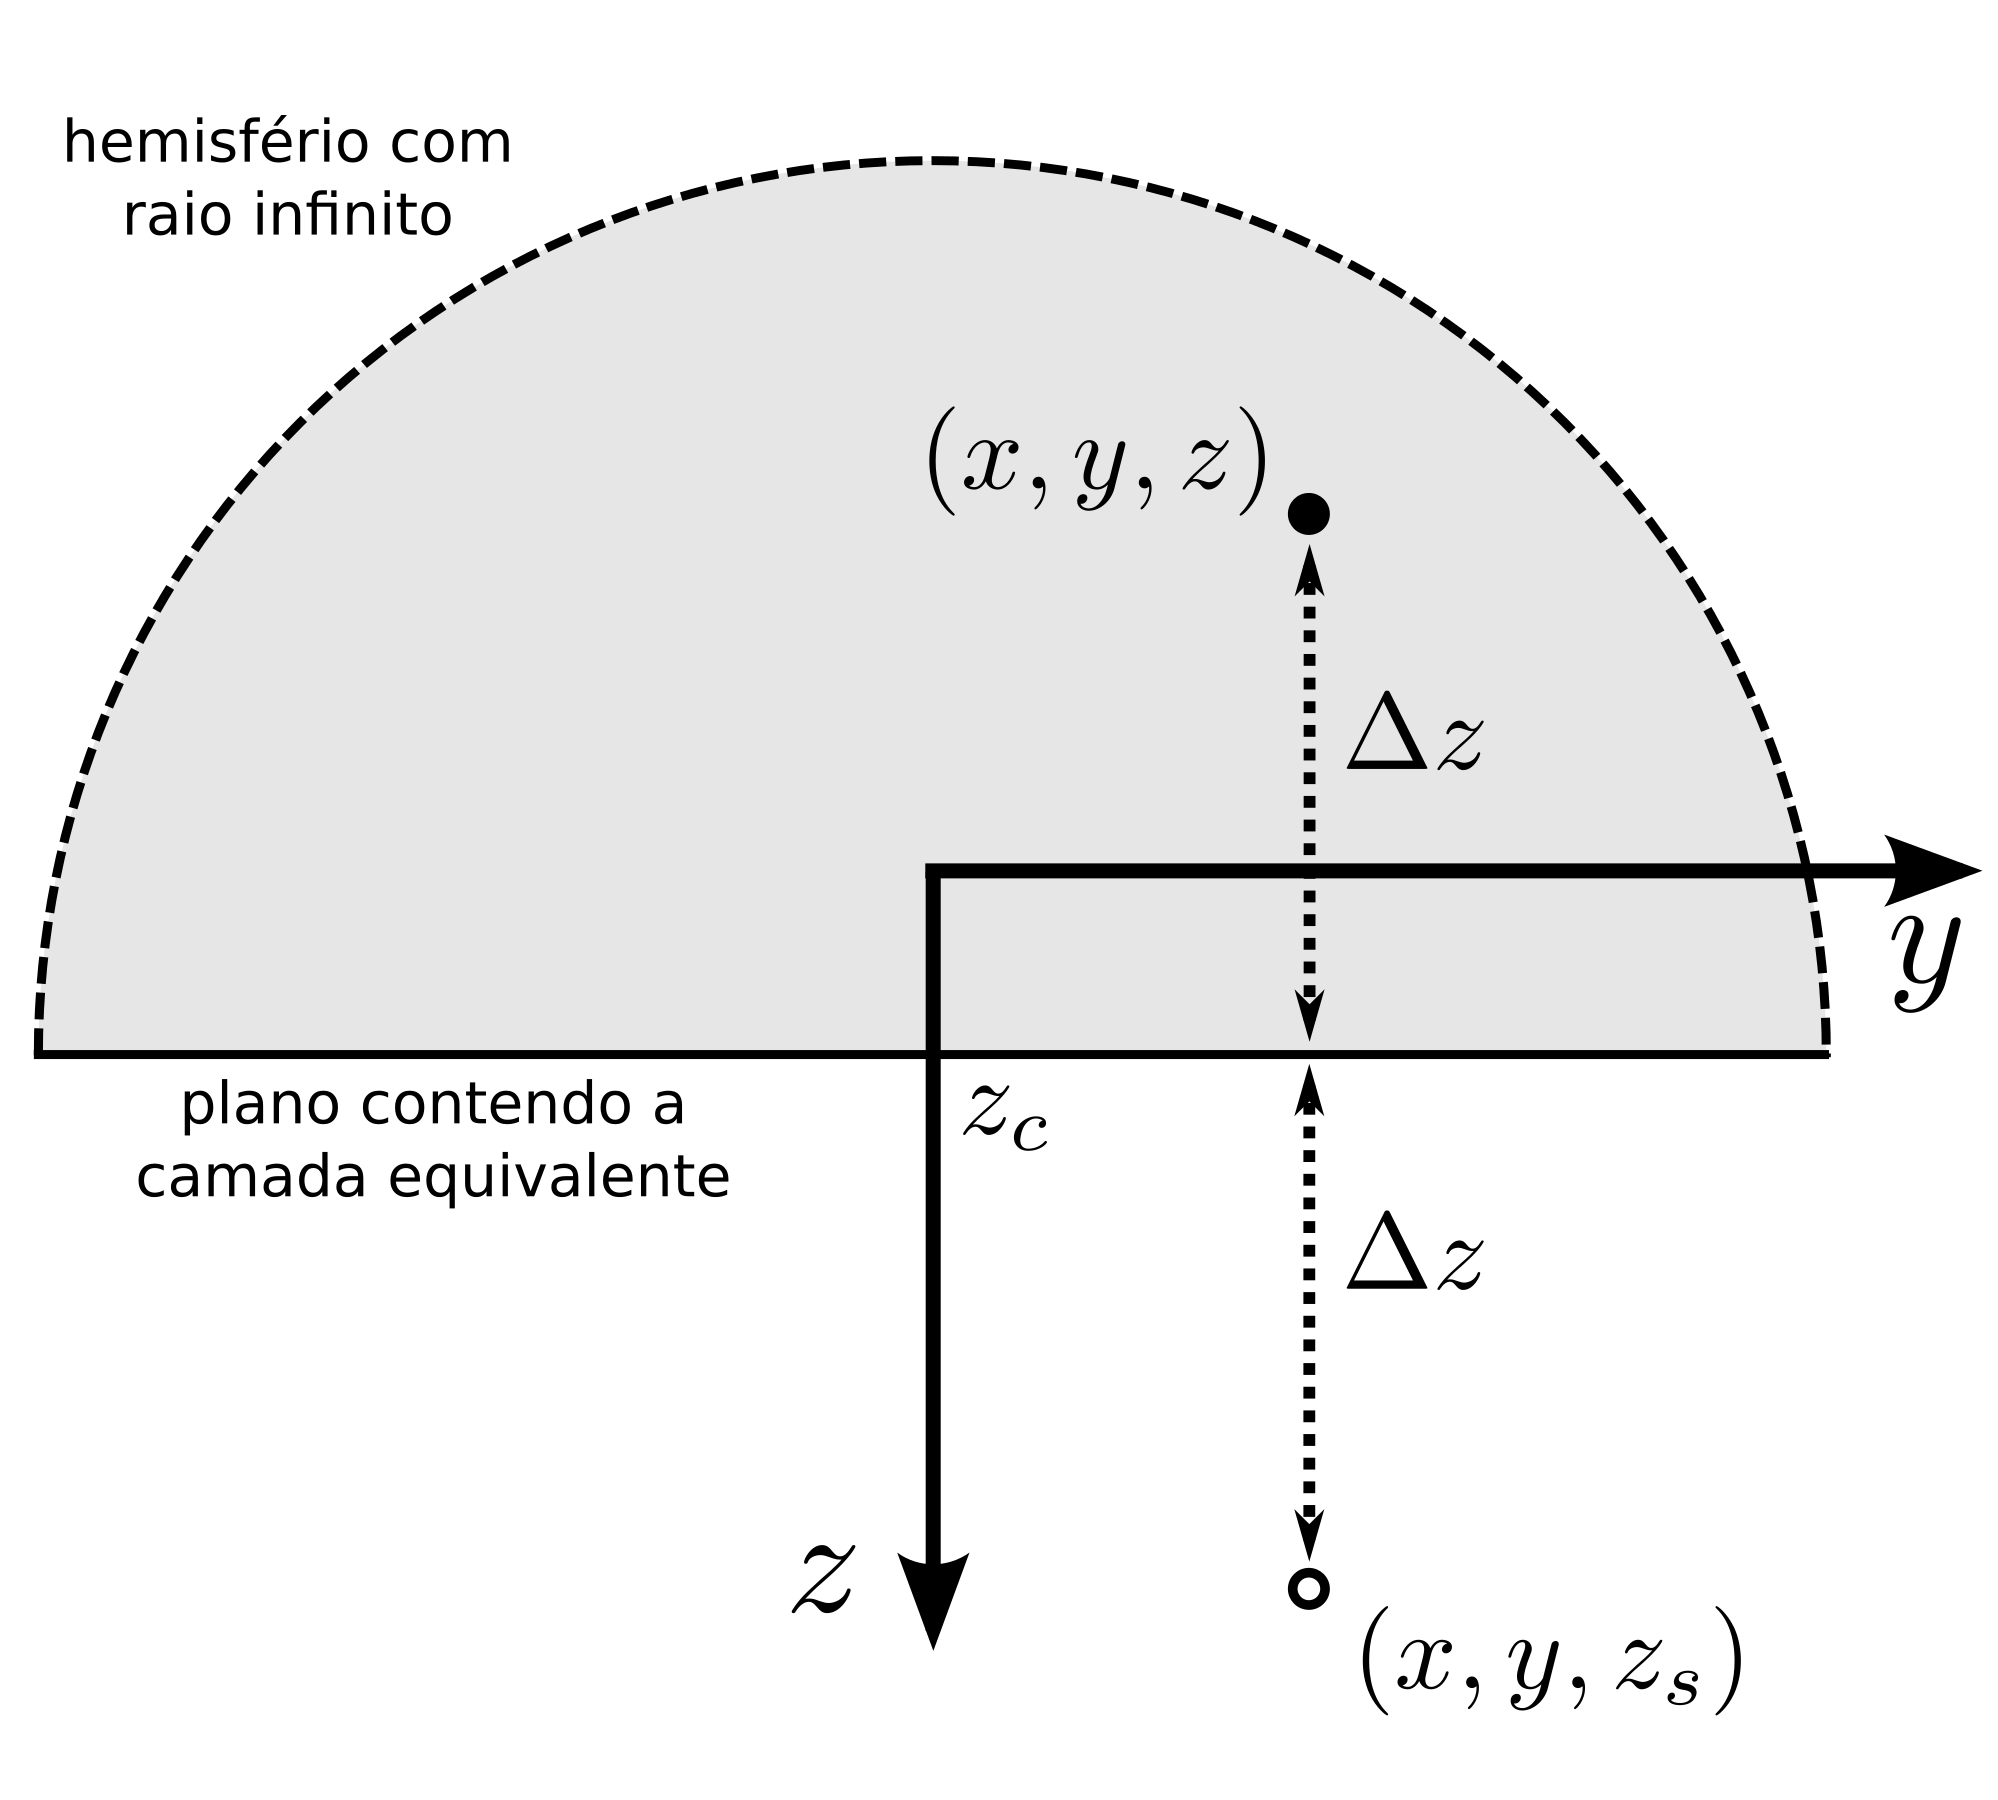
\includegraphics[width=0.75\textwidth]{Fig/eqlayer/surface_Green.png}
	\caption{ Representação 2D da superfície utilizada para aplicar as identidades de Green. A superfície é formada por uma semi-esfera (linha traçejada) com raio infinito e o plano $z = z_{c}$ contendo a camada equivalente. Os pontos $(x, y, z)$ (ponto fechado) e $(x, y, z_{s})$ (ponto aberto) são posicionados simetricamente com respeito ao plano $z = z_{c}$ e definidos como $z = z_{c} - \Delta z$ e $z = z_{c} + \Delta z$, respectivamente.}
	\label{fig:surface_Green}
\end{figure}